\documentclass[a4paper,twoside,anonymous]{article}

\usepackage[T1]{fontenc}
\usepackage{lmodern}%
%\usepackage{pgf-pie} % Para fazer gráfico de pizza 
\usepackage{tikz}{}
\usepackage{pgfplots}
\usepackage{gensymb} % Para o símbolo de grau º \degree
%PGPLOTS
\usetikzlibrary{patterns}
\usepgfplotslibrary[statistics] % ConTEXt
\usetikzlibrary{pgfplots.statistics} % LATEX and plain TEX
\usepackage{tikz}
\usepackage{ragged2e}
\pgfplotsset{width=9cm, height=8cm, compat=1.9}
\usetikzlibrary{patterns,arrows, shapes.geometric,calc}
\usepackage{gensymb}
\usepackage{threeparttable}
\usepackage{listings}
\usepackage{paralist} %inparaenum
\usepackage{adjustbox}
\usepackage{url}
\usepackage{xcolor,colortbl}
\usepackage{epsfig}
\usepackage{subcaption}
\usepackage{calc}
\usepackage{amssymb}
\usepackage{amstext}
\usepackage{amsmath}
\usepackage{amsthm}
\usepackage{multicol}
\usepackage{pslatex}
\usepackage{apalike}
\usepackage{SCITEPRESS}     % Please add other packages that you may need BEFORE the SCITEPRESS.sty package.

\tikzset{
  chart/.style={
    legend label/.style={font={\scriptsize},anchor=west,align=left},
    legend box/.style={rectangle, draw, minimum size=5pt},
    axis/.style={black,semithick,->},
    axis label/.style={anchor=east,font={\tiny}},
  },
  bar chart/.style={
    chart,
    bar width/.code={
        \pgfmathparse{##1/2}
        \global\let\bar@w\pgfmathresult
    },
    bar/.style={very thick, draw=white},
    bar label/.style={font={\bfseries\small},anchor=north},
    bar value/.style={font={\footnotesize}},
    bar width=.75,
  },
  pie chart/.style={
    chart,
    slice/.style={line cap=round, line join=round, very thick,draw=white},
    pie title/.style={font={\bfseries}},
    slice type/.style n args={3}{
        ##1/.style={pattern color=##2,pattern=##3},
        values of ##1/.style={}
    }
}}
\pgfdeclarelayer{background}
\pgfdeclarelayer{foreground}
\pgfsetlayers{background,main,foreground}


\newcommand{\pie}[3][]{
    \begin{scope}[#1]
    \pgfmathsetmacro{\curA}{90}
    \pgfmathsetmacro{\r}{1}
    \def\c{(0,0)}
    \node[pie title] at (90:1.3) {#2};
    \foreach \v/\s in{#3}{
        \pgfmathsetmacro{\deltaA}{\v/100*360}
        \pgfmathsetmacro{\nextA}{\curA + \deltaA}
        \pgfmathsetmacro{\midA}{(\curA+\nextA)/2}

        \path[slice,\s] \c
            -- +(\curA:\r)
            arc (\curA:\nextA:\r)
            -- cycle;
        \pgfmathsetmacro{\d}{max((\deltaA * -(.5/50) + 1) , .5)}

        \begin{pgfonlayer}{foreground}
        \path \c -- node[pos=\d,pie values,values of \s]{$\v\%$} +(\midA:\r);
        \end{pgfonlayer}

        \global\let\curA\nextA
    }
    \end{scope}
}

\newcommand{\legend}[2][]{
    \begin{scope}[#1]
    \path
        \foreach \n/\s in {#2}
            {
                  ++(0,-10pt) node[\s,legend box] {} +(5pt,0) node[legend label] {\n}
            }
    ;
    \end{scope}
}

\begin{document}

\title{Textual Approach for Designing Database Conceptual Models: \\A focus group}
%\title{Textual Approach to Database Design in a Modeling Tool: a Focus Group}

% \author{
% \authorname{First Author\sup{1}\orcidAuthor{0000-0000-0000-0000}, 
% Second Author\sup{1}\orcidAuthor{0000-0000-0000-0000},
% Third Author\sup{1}\orcidAuthor{0000-0000-0000-0000} and 
% Fourth Author\sup{1}\orcidAuthor{0000-0000-0000-0000}}
% \affiliation{\sup{1}Institute of Problem Solving, XYZ University, My Street, MyTown, MyCountry}
% \email{\{f\_author, s\_author\}@ips.xyz.edu, t\_author@dc.mu.edu}
% }

\author{\authorname{Jonnathan Lopes\sup{1}\orcidAuthor{0000-0001-9402-801X}, Maicon Bernardino\sup{1}\orcidAuthor{0000-0003-2776-8020}, Fábio Basso\sup{1}\orcidAuthor{0000-0003-4275-0638} and Elder Rodrigues\sup{1}\orcidAuthor{0000-0003-3431-2814}}  
\affiliation{\sup{1}Federal University of Pampa - PPGES - LESSE -
Av. Tiaraj\'u, 810 - Ibirapuit\~a, CEP 97546-550 - Alegrete - RS, Brazil}
\email{\{jonnathan.riquelmo, fabiopbasso, eldermr\}@gmail.com, bernardino@acm.org}
}

\keywords{Domain specific language, Conceptual data model, Conceptual model, Database modeling.}

%\abstract{The abstract should summarize the contents of the paper and should contain at least 70 and at most 200 words. The text must be set to 9-point font size.}
\abstract{
Different approaches to software development are based on at least three database models: conceptual, logical, and physical, requiring distinct abstraction levels to represent complementary concepts.
The selection of a conceptual database modeling approach, among other things, depends on the problem domain, knowledge, and preferences of the developer. 
% In this paper we introduce the ERtext, a new Domain-Specific Language (DSL) developed in conformance with the ECore metamodel with the aid of the Xtext.
%, an open-source framework for developing textual DSLs. 
This paper presents a new domain-specific textual language devoted to the conceptual relational database modeling, \textit{i.e.}, entity-relationship modeling. 
% Additionally, based on predefined assumptions, we generated a logical database model through a model-to-text transformation, which resulted in fourteen entities.
% This paper reports a running example of using our proposed textual language called ERtext, applied to represent a conceptual data model for the digital media store domain, which includes eleven entities and ten relationships, as well as a self-relationship and a ternary relationship.
Furthermore, we present a preliminary evaluation conducted to analyze our proposed DSL, comparing two grammar versions in a focus group research method.
}

\onecolumn \maketitle \normalsize \setcounter{footnote}{0} \vfill

%#######################################################
%#######################################################
\section{\uppercase{Introduction}} 
\label{sec:introduction}
%#######################################################%#######################################################

%##### ES -> bancos de dados
Software Engineering (SE) is not feasible without persistence and data manipulation.
%~\cite{Sommerville:2011}
According to Date~\cite{Date:1990}, a database is a collection of stored operational data, used by the application systems of some organization.
For Elmasri and Navathe~\cite{Elmasri:2015}, a database can be defined as an abstraction from the real world, also called the mini-world, since it represents aspects that, together, carry an implicit meaning.
%Analyzing more objectively, 
Databases can be considered as the most important organizational assets today.
This is due to the fact that they do not only store trivial information but, for instance, also billing data, market research, and other aspects assisting in decision making.

%##### Ensino de BD
In this scenario, it is notable that there is an increasing effort of academia to provide a good level of preparation for future professionals who will enter an increasingly demanding industry. 
Higher education institutions, \textit{e.g.} universities, often approach the database curriculum with specific courses converging in their programs.
The database teaching area is an essential part of computer professional training.
The focus on database teaching is generally divided into four stages: 
(i) design and modeling, 
(ii) database management systems, 
(iii) comparative studies among these systems, and 
(iv) the application development~\cite{Aldmour:2010,Connolly:2006}.

%##### Contribuir com uma solução para o processo ensino-aprendizagem
Assuming that there is a growing search for instruments supporting the teaching-learning process in academia, we present a study focusing on the first stage: design and modeling.
In general, teaching database design and modeling includes the presentation of essential topics and the subsequent introduction of modeling tools using generally graphic approaches.
While graphical modeling is the most popular approach, textual modeling can be an alternative to the teaching-learning process at a higher level~\cite{Dimitrieski:2015}. 
This is due to the lack of textual approaches for the first stage. Hence, this limitation can represent a gap in the teaching-learning process of database modeling.

Considering that logical and physical modeling occur mainly in text mode, an approach like the one adopted in the ERtext tool can be considered viable because it manages to maintain the same style workflow in all modeling stages.
Nowadays, the declarative programming using Domain-Specific Languages (DSLs)~\cite{Kelly08} is the dominant paradigm of an extensive set of domains, \textit{e.g.} databases or templating.
With this approach, instead of hundreds of lines of verbose code it is possible to make clearly defined data schemes, providing an abstract representation, semantically simpler and meaningful.
Built on a grammar perceived in the proposed study as ``ease to use'' and as ``useful'', the main aim of this paper is to report the ERtext, a modeling tool based on a DSL for the database designing and modeling with the scope in conceptual level modeling.

%##### Estrutura do artigo
This paper is organized as it follows.
Section \ref{sec:relatedWork} presents the related work. 
Section \ref{sec:analysisDesign} provides the design decisions and the architecture adopted. %for the proposal development
Section \ref{sec:ertextTool} describes an overview of the tool operation.
Finally, Section \ref{sec:conclusion} concludes this paper.

%########################################################
%########################################################
\section{\uppercase{Related Work}} 
\label{sec:relatedWork}
%########################################################
%########################################################

This section describes the most representative works for the object of this study: conceptual database modeling.
After an extensive study composed of a Multivocal Literature Mapping (MLM) (DOI: \url{doi.org/10.5281/zenodo.4064987} - in portuguese), we selected proposals and tools closely matching with our features from our DSL.

Dimitrieski \textit{et al.} \cite{Celikovic:2014,Dimitrieski:2015} presents a tool called System Modeling Tool (MIST).
This tool uses a DSL called EERDSL, a language based on the improved Extended Entity-Relationship (EER) model.
The EER includes all the concepts as extension from those introduced by the original ER model proposed by Chen \cite{Chen:1976}.
In addition, it includes the concepts of subclasses and superclasses (\textit{Is-a}), along with the concepts of specialization and generalization.
MIST presents a bidirectional (graphical and textual) modeling approach for the data model approach. 
%The author argues that this decision is based on the following understanding: the preference for the modeling approach used may depend on the problem domain, knowledge, and personal preferences of a database designer. 
%It also presents a previous experience, in which a modeling tool was built with a forms-based approach. 
From the results obtained, the idea of MIST was conceived.
The purpose of the tool is to apply it both in the professional market and for teaching designing and modeling databases in the academic environment. 
MIST was developed with the aid of the Xtext framework for the notation of textual DSL and initially used the Eugene framework, a project that was discontinued, for its graphic version. 
As a result, Eugene was replaced by the Sirius framework. Besides, MIST also supports the generation of SQL code.

Dbdiagram.io (\url{https://dbdiagram.io/})
%\footnote{Dbdiagram.io:\url{https://dbdiagram.io/}} 
is a web-based open-source tool for drawing an Entity Relationship Diagram (ERD), with a textual approach implementing its own DSL.
This DSL uses a model similar to the logic view, with a differential of fast learning curve and, in addition, an intuitive graphical representation.
The presentation of the diagram elements can be freely organized by the user in real time.
However, it is worth to note that all modeling is in fact performed in a textual manner.
Moreover, the tool also offers automatic generation of SQL code.

Likewise, QuickDBD %(\url{https://quickdatabasediagrams.com/})
%\footnote{QuickDBD: \url{https://quickdatabasediagrams.com/}} 
is a web-based tool adopting  the same operational mode as dbdiagram.io, also implementing its own textual DSL for database modeling.
However, it is a proprietary tool, \textit{i.e.} paid for and with an explicit focus on the industry.
Both tools are also very similar to the generation of graphical model representations and highlight several arguments for their adoption, such as the quick understanding of their DSL, the perspective of carrying out fluid works, the access of any platform and design sharing.

Finally, the web-based open-source tool RelaX (Relational Algebra Calculator)~\cite{Kessler:2019}
%\footnote{RelaX: \url{https://dbis-uibk.github.io/relax/}}.
%This tool was not found in our systematic mapping, but indicated by a researcher of DSL and database areas.
is developed in the academic environment aiming at teaching relational algebra through operations on relational databases.
It has a textual approach, using a DSL called RelAlg, and including two operational perspectives: RelAlg and SQL commands.
RelaX uses a model approach already at a physical level for operations, such as DDLs for data structures and DMLs for data manipulation \textit{e.g.} queries.
%such as Data Definition Languages (DDLs) for data structures and Data Manipulation Languages (DMLs) for data manipulation \textit{e.g.} queries.
Despite its functionality, RelaX is not built as a database designing and modeling tool, but it intents for use restricted for teaching in the academic environment.

Several different tools have been put forward, the main difference from ERText is that the related work focuses in the logical or in physical model design. 
MIST on the other hand aims at the conceptual model, and since it was not possible to find the tool, or at least its code, for an analysis of usage, unlike Dbdiagram.io, QuickDBD and RelaX, we cannot properly compare MIST with ERText. 
This highlights another important difference, since our proposal is completely open-source, available for use, evaluation and learning. 
Among the mentioned tools, only RelaX has its code also available.
This may indicate that the general applicability of our tool in the teaching-learning process of database  conceptual modeling in the academic is possibly greater than these tools.

%#################################################
%#################################################
\section{\uppercase{Analysis and Design}}
\label{sec:analysisDesign}
%#################################################
%#################################################

This section presents the analysis and designing phases, describing the requirements raised for the DSL definition and its associated design decisions as well as the grammar and the architecture are shown.
%Afterward, the grammar and the architecture are shown.

%#################################################
\subsection{Software Requirements} \label{sec:reqDSL}
%#################################################

Our focus is on the teaching process, so it is essential to tag ERText as an open-source license, allowing the evolution and collaborative maintenance with the involvement of other developers.

In the following, we listed the Software Requirements (SR) that were defined based on the surveyed literature: %, as well as the prior knowledge of the researchers involved in conducting the study.
%\begin{inparadesc}
% \begin{inparaenum}
%\item
\textbf{SR1.} DSL must be made available under an open-source license.
%\item 
\textbf{SR2.} The DSL should allow for the textual representation of conceptual data models.
% As it is an objective that the solution be another option in relation to graphical approaches, this requirement is justified.
% This allows you to focus on understanding the domain and developing DSL.
%\item 
\textbf{SR3.} Conceptual data models should support the definition of fundamental domain concepts such as entities, attributes, relationships, and their cardinalities.
% Conceptual data models should support the definition of entities, attributes, relationships and cardinalities
% The tools used for language development need to allow the domain concepts that govern the traditional ERD structure to be implemented.
%\item 
\textbf{SR4.} Conceptual data models should support the definition of attributes, identifiers, generalization and specialization, self-relationships, and ternary relationships.
% The language should allow more sophisticated concepts of the domains to be defined.
%\item 
\textbf{SR5.} DSL implementation must transform from the conceptual to the logical model displaying the result generated to the user.
% The language must perform the transformation from conceptual to logical models, displaying the result generated to the user.
% \end{inparaenum}
%\end{inparadesc}

%#################################################
%\subsection{Design Decisions} \label{sec:decDSL}
%#################################################

In the following we described the Design Decisions (DD) supporting all the previously discussed SRs:
%
%\begin{inparadesc}
    %\item 
    \textbf{DD1.} The solution must adopt an open-source LW (Language Workbench) to aid the implementation of the textual DSL (SR1, SR2).
    Through the investigation conducted during this study, we select the LW Xtext for the development of our DSL. %as it is an open-source framework focused on the development of textual DSLs, providing all the necessary features and infrastructure. In addition, Xtext is a tool with a high level of maturity, detailed documentation, and an active user community.
    %\item 
    \textbf{DD2.} A DSL must provide a textual representation  equivalent to the currently graphical ER model (SR3, SR4).
    For the SRs covered by this DD, we adopted a strategy to carry out an analysis on the tools identified in an MLM,
    % a multivocal literature mapping, 
    as well as in the Heuser's reference book~\cite{Heuser:2009}.
    %\item 
    \textbf{DD3.} The solution must perform the transformation among the models (\textit{e.g.} conceptual, logical, and physical) (SR5).
    %Xtext uses the Eclipse Modeling Framework (EMF) models as the in-memory representation of any analyzed text file.
    %This graph of objects in memory is called the Abstract Syntactic Tree (AST).
    %These concepts are also called Document Object Model (DOM), semantic model, or simply model.
    %There is a representation of the grammar model in the form of a central metamodel in the EMF core, called the ECore model.
    %Hence, having the proposed DSL ECore as a representation, it is then possible to apply transformation rules, thus generating other models.
%\end{inparadesc}

%#################################################
\subsection{The Language} \label{sec:EspecDSL}
%#################################################

\definecolor{javared}{rgb}{0.6,0,0} % for strings
\definecolor{javagreen}{rgb}{0.25,0.5,0.35} % comments
\definecolor{javapurple}{rgb}{0.5,0,0.35} % keywords
\definecolor{javadocblue}{rgb}{0.25,0.35,0.75} % javadoc
\definecolor{verde}{rgb}{0.25,0.5,0.35}
\definecolor{jpurple}{rgb}{0.5,0,0.35}
\definecolor{darkgreen}{rgb}{0.0, 0.2, 0.13}


\lstdefinelanguage{Xtext}{
  sensitive = true,
  keywords={},
  keywords=[2]{ERModel, Domain, Attribute, Entity, Relation, RelationSide, DataType, CardinalityType},
  keywords=[3]{grammar, with, generate, Terminals, enum},
  otherkeywords={*, ?, +, *=, ?=, +=, |},
  keywordstyle=\color{black}\bfseries,
  keywordstyle=[2]\color{javadocblue}\bfseries,
  keywordstyle=[3]\color{javapurple}\bfseries,% for example
%   backgroundcolor=\color{cyan!10},
%   numbers=left,
%   stepnumber=1,
  numbersep=8pt,
  showstringspaces=false,
  breaklines=true,
  frame=top,
  comment=[l]{//},
  morecomment=[s]{/*}{*/},
  commentstyle=\color{black}\ttfamily, 
%   \ttfamily \bfseries
  stringstyle=\color{javared},
  morestring=[b]',
  morestring=[b]"
  }
  
  \lstdefinelanguage{Xtext2}{
  sensitive = true,
  keywords={},
  keywords=[2]{ERModel, Domain, Attribute, Entity, Relation, RelationSide, DataType, CardinalityType},
  keywords=[3]{grammar, with, generate, Terminals, enum},
  otherkeywords={*, ?, +, *=, ?=, +=, |},
  keywordstyle=\color{black}\bfseries,
  keywordstyle=[2]\color{javadocblue}\bfseries,
  keywordstyle=[3]\color{javapurple}\bfseries,% for example
  backgroundcolor=\color{cyan!10},
  numbers=left,
  stepnumber=1,
  numbersep=8pt,
  showstringspaces=false,
  breaklines=true,
  frame=top,
  comment=[l]{//},
  morecomment=[s]{/*}{*/},
  commentstyle=\color{black}\ttfamily,
  stringstyle=\color{javared}\ttfamily,
  morestring=[b]',
  morestring=[b]"
  }
  
  \lstdefinelanguage{ERDSL}{
  sensitive = true,
  keywords={},
  keywords=[2]{Domain, Entities, Relationships, isIdentifier, isRelatedWith, isA, zero, one, many},
  keywords=[3]{int, money, string, datetime, file},
  otherkeywords={*, ?, +, *=, ?=, +=, |},
  keywordstyle=\color{black}\bfseries,
  keywordstyle=[2]\color{javapurple}\bfseries,
  keywordstyle=[3]\color{javadocblue}\bfseries,% for example
%   backgroundcolor=\color{cyan!10},
%   numbers=left,
%   stepnumber=1,
  captionpos=t,
  numbersep=8pt,
  showstringspaces=false,
  breaklines=true,
  frame=top,
  comment=[l]{//},
  morecomment=[s]{/*}{*/},
  commentstyle=\color{black}\ttfamily,
  stringstyle=\color{javared}\ttfamily,
  morestring=[b]',
  morestring=[b]"
  }
  
  \lstdefinelanguage{BNF}{
  sensitive = true,
  keywords={},
  keywords=[2]{},
  otherkeywords={::= , |, <, >},
  keywordstyle=\color{javapurple}\bfseries,
  keywordstyle=[2]\color{javapurple}\bfseries,
  keywordstyle=[3]\color{javadocblue}\bfseries,% for example
%   backgroundcolor=\color{cyan!10},
%   numbers=left,
%   stepnumber=1,
  captionpos=t,
  numbersep=8pt,
  showstringspaces=false,
  breaklines=true,
  frame=top,
  comment=[l]{//},
  morecomment=[s]{/*}{*/},
  commentstyle=\color{darkgreen}\ttfamily,
  stringstyle=\color{javared}\ttfamily,
  morestring=[b]',
  morestring=[b]"
  }
  
  
  
  

In the current phase of the work, the language at the conceptual level is not fully finalized.
There are topics related to the scope validation, as in the case of the treatment of unwanted cross-references and other restrictions inherent to the ER model that must be analyzed and then implemented.
The grammar definition of the created DSL is displayed in Figure \ref{fig:DSLvsFinal}.

% basicstyle=\linespread{0.83}\small\ttfamily, % Global Code Style
% literate=*{*}{\normalfont{*}}1,
% morecomment=[l][\color{singleLineCommentColor}]{//},
% morecomment=[s][\color{multiLineCommentColor}]{/*}{*/},
% morestring=[b]",
% morestring=[b]',
% commentstyle=\color{commentColor},
% keywordstyle=[1]{\bfseries\color{keyword1Color}},
% keywordstyle=[2]{\bfseries\color{keyword2Color}},
% stringstyle=\color{stringColor},
% %...

\lstset{
basicstyle=\scriptsize,
literate={% replace strings with symbols
    {->}{{$\to$}}{2}
    {*}{\textasteriskcentered}{1}
    %{'}{\textquotesingle}{1}
  }
}

\begin{figure}[!htb]
    \centering
    \begin{scriptsize}
    \begin{lstlisting}[basicstyle = \tiny, language = Xtext, frame = trbl]
grammar org.xtext.university.ertext.ERtext 
with org.eclipse.xtext.common.Terminals
generate ERtext "http://www.xtext.org/unipampa/ertext/ERtext"
ERModel:
    domain=Domain ';'
    ('Entities' '{') entities+=Entity+ ('}' ';')
    ('Relationships' '{') relations+=Relation*
       ('}' ';');
Domain:
    'Domain' name=ID;
Attribute:
    name=ID type=DataType (isKey?='isIdentifier')?;
Entity:
    name=ID ('is' is+=[Entity])*
    ('{' attributes+=Attribute
    (',' attributes+=Attribute)*'}')?;
Relation:
    (name=ID)? ('[' leftEnding=RelationSide 
    'relates' 
    rightEnding=RelationSide ']') 
    ('{' attributes+=Attribute 
    (',' attributes+=Attribute)* '}')*;
RelationSide:
    cardinality=('(0:1)'|'(1:1)'|'(0:N)'|'(1:N)') 
    target=[Entity] | target=[Relation];
enum DataType:
    INT='int'           | DOUBLE='double'       | 
    MONEY='money'       | STRING='string'       |
    BOOLEAN='boolean'   | DATETIME='datetime'   |
    BLOB='file';
    \end{lstlisting}
    \end{scriptsize}
    \caption{Grammar definition of the DSL.}
    \label{fig:DSLvsFinal}
\end{figure}

The \texttt{grammar} command specifies the DSL name, while the \texttt{with} statement declares an inheritance from another language.
In the case of the proposed grammar, a standard Xtext grammar, called \texttt{Terminals}, will be used, which provides some predefined rules
%, \textit{e.g.} the rule \texttt{ID} for identifiers or \texttt{INT} for integers.
The \texttt{generate} command is the statement that produces the language's AST.

The first rule, called the input rule, defines what the general language structure looks like.
Words and symbols in double or single quotes indicate reserved words.
For example, the object \texttt{Entities} must be preceded by ``\texttt {Entities \{}''.
This object represents a kind of container as indicated through the assignment operator \texttt{+=}.
It is an object that can contains other objects, in this case, one or more \texttt{Entity}.
It is established that each DSL file must also be composed of a \texttt{Domain} and zero or more \texttt{Relation} objects.

For a better understanding, it should be made clear that multiplicity is indicated by \texttt{*} (zero or many), \texttt{+} (one or many), or \texttt{?} (zero or one).
By not placing any of these operators, then one implicitly is expected to occur.
Regarding assignments, when only one \texttt{=} is specified it means that the object on the left expects only one record.
Therefore, for \texttt{+=} then zero, one or more occurrences are expected.

The \texttt{Domain} object is preceded by a reserved word with the same name, followed by an identifier.
The entity is defined by the \texttt{Entity} statement and an identifier name for this object.
Defining an inheritance is optional using the reserved word \texttt{is}.
After defining the name, a body of keys opens in which the entity attributes are specified.
An entity must contain at least one attribute and, due to the possible existence of weak entity set, it does not need to be an identifier.

The compound rules are only performed due to the possibility of grouping expressions using parentheses, in addition to the possibility of using other rules through cross-references.
The brackets between the \texttt{Entity} rule are used to indicate that you want to use only the \texttt{name} attribute that identifies the object.
Entity attributes are defined by a name, inheriting the \texttt{ID} rule from \texttt{Terminals}, and optional attributes \textit{e.g.} \texttt{isIdentifier} to symbolize primary keys.

The relationship is defined, already within the body of the \texttt{Relationships} block, with an optional declaration of its identification.
Then, brackets are opened and two elements must be specified \texttt{RelationSide} as a reference to the attributes \texttt{leftEnding} and \texttt{rightEnding}.
These attributes represent the sides of a relationship.
These objects must be separated by the expression \texttt{relates}.
The sides of the relation are defined in the rule \textit{RelationSide}, composed of two attributes.
The \texttt{cardinality} attribute is mandatory and uses numerals \texttt{(0:1), (1:1), (0:N), (1:N)}.
The \texttt{target} attribute is likewise mandatory, accepting a cross-reference to a \texttt{Entity} or \texttt{Relation}.
In the case of a \texttt{target} referencing a \texttt{Relation}, then a ternary relationship is highlighted.
The attribute types are contained in an enumerated list called \texttt{DataType}, on the left is the representation in the model \textit{ECore}.
On the right is the reserved word that is used in the language.
The conditional symbol \texttt{|} means the logical operator \textit{OR} and serves to separate each definition \texttt{<key> = <value>} as an option within the list.

%#################################################
\subsection{Tool Architecture} \label{sec:arqDSL}
%#################################################

The solution architecture is shown in Figure \ref{fig:arqXtext} and was built with the help of Xtext, which helped to generate most of the editor's infrastructure, the parser and ECore model i.e., a representation in memory at runtime of the model created using DSL.
%Then, there were some necessary manual adjustments and the addition of the writing of a generator for the conversion from conceptual data models to logical data models.

\begin{figure}[!htb]
    \centering
    
\tikzset{every picture/.style={line width=0.75pt}} %set default line width to 0.75pt        

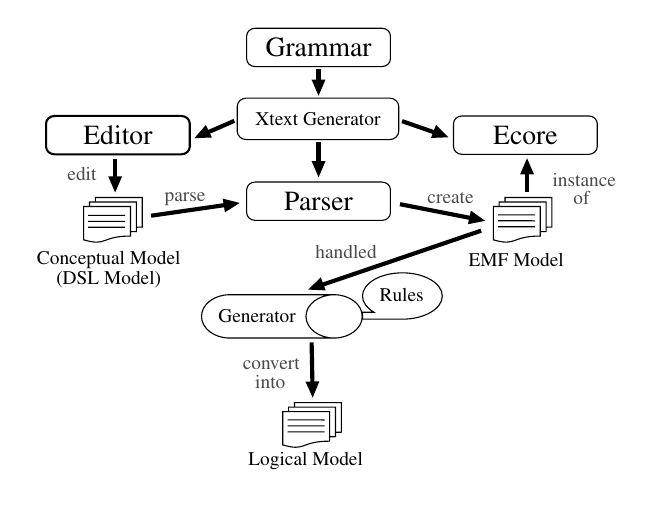
\begin{tikzpicture}[x=0.50pt,y=0.45pt,yscale=-1,xscale=1]
%uncomment if require: \path (0,465); %set diagram left start at 0, and has height of 465

%Rounded Rect [id:dp8080613887465731] 
\draw  [fill={rgb, 255:red, 255; green, 255; blue, 255 }  ,fill opacity=1 ] (166.24,24.37) .. controls (166.24,20.97) and (169,18.21) .. (172.4,18.21) -- (263.96,18.21) .. controls (267.36,18.21) and (270.11,20.97) .. (270.11,24.37) -- (270.11,42.84) .. controls (270.11,46.24) and (267.36,49) .. (263.96,49) -- (172.4,49) .. controls (169,49) and (166.24,46.24) .. (166.24,42.84) -- cycle ;
%Rounded Rect [id:dp23877247410758984] 
\draw  [fill={rgb, 255:red, 255; green, 255; blue, 255 }  ,fill opacity=1 ][line width=0.75]  (21.24,94.82) .. controls (21.24,91.42) and (24,88.66) .. (27.4,88.66) -- (118.95,88.66) .. controls (122.36,88.66) and (125.11,91.42) .. (125.11,94.82) -- (125.11,113.3) .. controls (125.11,116.7) and (122.36,119.46) .. (118.95,119.46) -- (27.4,119.46) .. controls (24,119.46) and (21.24,116.7) .. (21.24,113.3) -- cycle ;
%Flowchart: Multidocument [id:dp49717070559395604] 
\draw  [fill={rgb, 255:red, 255; green, 255; blue, 255 }  ,fill opacity=1 ] (56.88,154.12) -- (90.75,154.12) -- (90.75,177.89) .. controls (69.58,177.89) and (73.82,186.46) .. (56.88,180.91) -- cycle ; \draw  [fill={rgb, 255:red, 255; green, 255; blue, 255 }  ,fill opacity=1 ] (52.64,157.72) -- (86.52,157.72) -- (86.52,181.49) .. controls (65.35,181.49) and (69.58,190.06) .. (52.64,184.52) -- cycle ; \draw  [fill={rgb, 255:red, 255; green, 255; blue, 255 }  ,fill opacity=1 ] (48.41,161.32) -- (82.28,161.32) -- (82.28,185.09) .. controls (61.11,185.09) and (65.35,193.66) .. (48.41,188.12) -- cycle ;
%Straight Lines [id:da5642847406466045] 
\draw [fill={rgb, 255:red, 255; green, 255; blue, 255 }  ,fill opacity=1 ]   (51.63,168.47) -- (78.34,168.5) ;
%Straight Lines [id:da9779186616916171] 
\draw [fill={rgb, 255:red, 255; green, 255; blue, 255 }  ,fill opacity=1 ]   (51.63,173.26) -- (78.34,173.28) ;
%Straight Lines [id:da8217185402464098] 
\draw [fill={rgb, 255:red, 255; green, 255; blue, 255 }  ,fill opacity=1 ]   (51.63,178.04) -- (78.34,178.06) ;

%Straight Lines [id:da27204357118531197] 
\draw [fill={rgb, 255:red, 255; green, 255; blue, 255 }  ,fill opacity=1 ][line width=1.5]    (71.18,123.3) -- (71.18,146.06) ;
\draw [shift={(71.18,150.06)}, rotate = 270] [fill={rgb, 255:red, 0; green, 0; blue, 0 }  ][line width=0.08]  [draw opacity=0] (11.61,-5.58) -- (0,0) -- (11.61,5.58) -- cycle    ;
%Rounded Rect [id:dp014713549076222021] 
\draw  [fill={rgb, 255:red, 255; green, 255; blue, 255 }  ,fill opacity=1 ] (159.43,80.98) .. controls (159.43,77.3) and (162.41,74.31) .. (166.09,74.31) -- (269.45,74.31) .. controls (273.13,74.31) and (276.11,77.3) .. (276.11,80.98) -- (276.11,100.98) .. controls (276.11,104.66) and (273.13,107.65) .. (269.45,107.65) -- (166.09,107.65) .. controls (162.41,107.65) and (159.43,104.66) .. (159.43,100.98) -- cycle ;
%Rounded Rect [id:dp8159423215616721] 
\draw  [fill={rgb, 255:red, 255; green, 255; blue, 255 }  ,fill opacity=1 ] (315.72,94.82) .. controls (315.72,91.42) and (318.48,88.66) .. (321.88,88.66) -- (413.44,88.66) .. controls (416.84,88.66) and (419.59,91.42) .. (419.59,94.82) -- (419.59,113.3) .. controls (419.59,116.7) and (416.84,119.46) .. (413.44,119.46) -- (321.88,119.46) .. controls (318.48,119.46) and (315.72,116.7) .. (315.72,113.3) -- cycle ;
%Flowchart: Multidocument [id:dp814245162277164] 
\draw  [fill={rgb, 255:red, 255; green, 255; blue, 255 }  ,fill opacity=1 ] (352.96,154.12) -- (386.83,154.12) -- (386.83,177.89) .. controls (365.66,177.89) and (369.89,186.46) .. (352.96,180.91) -- cycle ; \draw  [fill={rgb, 255:red, 255; green, 255; blue, 255 }  ,fill opacity=1 ] (348.72,157.72) -- (382.6,157.72) -- (382.6,181.49) .. controls (361.43,181.49) and (365.66,190.06) .. (348.72,184.52) -- cycle ; \draw  [fill={rgb, 255:red, 255; green, 255; blue, 255 }  ,fill opacity=1 ] (344.49,161.32) -- (378.36,161.32) -- (378.36,185.09) .. controls (357.19,185.09) and (361.43,193.66) .. (344.49,188.12) -- cycle ;
%Straight Lines [id:da659202853659377] 
\draw [fill={rgb, 255:red, 255; green, 255; blue, 255 }  ,fill opacity=1 ]   (347.97,168.04) -- (374.69,168.06) ;
%Straight Lines [id:da8271632436642871] 
\draw [fill={rgb, 255:red, 255; green, 255; blue, 255 }  ,fill opacity=1 ]   (347.97,172.82) -- (374.69,172.85) ;
%Straight Lines [id:da22701123408508272] 
\draw [fill={rgb, 255:red, 255; green, 255; blue, 255 }  ,fill opacity=1 ]   (347.97,177.61) -- (374.69,177.63) ;

%Straight Lines [id:da6612735011438882] 
\draw [fill={rgb, 255:red, 255; green, 255; blue, 255 }  ,fill opacity=1 ][line width=1.5]    (368.86,126.65) -- (368.86,149.4) ;
\draw [shift={(368.86,122.65)}, rotate = 90] [fill={rgb, 255:red, 0; green, 0; blue, 0 }  ][line width=0.08]  [draw opacity=0] (11.61,-5.58) -- (0,0) -- (11.61,5.58) -- cycle    ;
%Rounded Rect [id:dp9641259565957541] 
\draw  [fill={rgb, 255:red, 255; green, 255; blue, 255 }  ,fill opacity=1 ] (166.24,147.89) .. controls (166.24,144.48) and (169,141.73) .. (172.4,141.73) -- (263.96,141.73) .. controls (267.36,141.73) and (270.11,144.48) .. (270.11,147.89) -- (270.11,166.36) .. controls (270.11,169.76) and (267.36,172.52) .. (263.96,172.52) -- (172.4,172.52) .. controls (169,172.52) and (166.24,169.76) .. (166.24,166.36) -- cycle ;
%Straight Lines [id:da4555835119587406] 
\draw [fill={rgb, 255:red, 255; green, 255; blue, 255 }  ,fill opacity=1 ][line width=1.5]    (218.18,50.89) -- (218.18,68.42) ;
\draw [shift={(218.18,72.42)}, rotate = 270] [fill={rgb, 255:red, 0; green, 0; blue, 0 }  ][line width=0.08]  [draw opacity=0] (11.61,-5.58) -- (0,0) -- (11.61,5.58) -- cycle    ;
%Straight Lines [id:da2586670416419199] 
\draw [fill={rgb, 255:red, 255; green, 255; blue, 255 }  ,fill opacity=1 ][line width=1.5]    (218.18,109.78) -- (218.18,133.88) ;
\draw [shift={(218.18,137.88)}, rotate = 270] [fill={rgb, 255:red, 0; green, 0; blue, 0 }  ][line width=0.08]  [draw opacity=0] (11.61,-5.58) -- (0,0) -- (11.61,5.58) -- cycle    ;
%Straight Lines [id:da2552674310073062] 
\draw [fill={rgb, 255:red, 255; green, 255; blue, 255 }  ,fill opacity=1 ][line width=1.5]    (157.32,92.59) -- (132.04,104.77) ;
\draw [shift={(128.43,106.51)}, rotate = 334.28] [fill={rgb, 255:red, 0; green, 0; blue, 0 }  ][line width=0.08]  [draw opacity=0] (11.61,-5.58) -- (0,0) -- (11.61,5.58) -- cycle    ;
%Straight Lines [id:da29550662771480396] 
\draw [fill={rgb, 255:red, 255; green, 255; blue, 255 }  ,fill opacity=1 ][line width=1.5]    (308.34,104.31) -- (278.52,92.81) ;
\draw [shift={(312.07,105.76)}, rotate = 201.11] [fill={rgb, 255:red, 0; green, 0; blue, 0 }  ][line width=0.08]  [draw opacity=0] (11.61,-5.58) -- (0,0) -- (11.61,5.58) -- cycle    ;
%Straight Lines [id:da3280771928101003] 
\draw [fill={rgb, 255:red, 255; green, 255; blue, 255 }  ,fill opacity=1 ][line width=1.5]    (97.15,168.77) -- (157.22,159.13) ;
\draw [shift={(161.17,158.5)}, rotate = 530.89] [fill={rgb, 255:red, 0; green, 0; blue, 0 }  ][line width=0.08]  [draw opacity=0] (11.61,-5.58) -- (0,0) -- (11.61,5.58) -- cycle    ;
%Straight Lines [id:da9478402467031726] 
\draw [fill={rgb, 255:red, 255; green, 255; blue, 255 }  ,fill opacity=1 ][line width=1.5]    (277.03,159.51) -- (334.63,172.02) ;
\draw [shift={(338.54,172.87)}, rotate = 192.26] [fill={rgb, 255:red, 0; green, 0; blue, 0 }  ][line width=0.08]  [draw opacity=0] (11.61,-5.58) -- (0,0) -- (11.61,5.58) -- cycle    ;
%Flowchart: Direct Access Storage [id:dp7657317583515377] 
\draw  [fill={rgb, 255:red, 255; green, 255; blue, 255 }  ,fill opacity=1 ] (229.43,266.99) -- (153.92,266.99) .. controls (142.69,266.99) and (133.59,259.2) .. (133.59,249.6) .. controls (133.59,240) and (142.69,232.21) .. (153.92,232.21) -- (229.43,232.21)(249.75,249.6) .. controls (249.75,259.2) and (240.65,266.99) .. (229.43,266.99) .. controls (218.2,266.99) and (209.1,259.2) .. (209.1,249.6) .. controls (209.1,240) and (218.2,232.21) .. (229.43,232.21) .. controls (240.65,232.21) and (249.75,240) .. (249.75,249.6) ;
%Straight Lines [id:da100480350897858] 
\draw [fill={rgb, 255:red, 255; green, 255; blue, 255 }  ,fill opacity=1 ][line width=1.5]    (335.65,180.79) -- (214.46,226.67) ;
\draw [shift={(210.72,228.08)}, rotate = 339.27] [fill={rgb, 255:red, 0; green, 0; blue, 0 }  ][line width=0.08]  [draw opacity=0] (11.61,-5.58) -- (0,0) -- (11.61,5.58) -- cycle    ;
%Flowchart: Multidocument [id:dp5253239734010293] 
\draw  [fill={rgb, 255:red, 255; green, 255; blue, 255 }  ,fill opacity=1 ] (200.79,318.82) -- (234.67,318.82) -- (234.67,342.59) .. controls (213.5,342.59) and (217.73,351.16) .. (200.79,345.61) -- cycle ; \draw  [fill={rgb, 255:red, 255; green, 255; blue, 255 }  ,fill opacity=1 ] (196.56,322.42) -- (230.44,322.42) -- (230.44,346.19) .. controls (209.26,346.19) and (213.5,354.76) .. (196.56,349.21) -- cycle ; \draw  [fill={rgb, 255:red, 255; green, 255; blue, 255 }  ,fill opacity=1 ] (192.32,326.02) -- (226.2,326.02) -- (226.2,349.79) .. controls (205.03,349.79) and (209.26,358.36) .. (192.32,352.81) -- cycle ;
%Straight Lines [id:da29635223798470123] 
\draw [fill={rgb, 255:red, 255; green, 255; blue, 255 }  ,fill opacity=1 ]   (195.81,332.74) -- (222.53,332.76) ;
%Straight Lines [id:da45709195099870326] 
\draw [fill={rgb, 255:red, 255; green, 255; blue, 255 }  ,fill opacity=1 ]   (195.81,337.52) -- (222.53,337.54) ;
%Straight Lines [id:da9397926099052756] 
\draw [fill={rgb, 255:red, 255; green, 255; blue, 255 }  ,fill opacity=1 ]   (195.81,342.31) -- (222.53,342.33) ;


%Straight Lines [id:da10826901476686546] 
\draw [fill={rgb, 255:red, 255; green, 255; blue, 255 }  ,fill opacity=1 ][line width=1.5]    (213.16,270.55) -- (213.89,310.78) ;
\draw [shift={(213.96,314.78)}, rotate = 268.97] [fill={rgb, 255:red, 0; green, 0; blue, 0 }  ][line width=0.08]  [draw opacity=0] (11.61,-5.58) -- (0,0) -- (11.61,5.58) -- cycle    ;
%Flowchart: Sequential Access Storage [id:dp3007368871754543] 
\draw  [fill={rgb, 255:red, 255; green, 255; blue, 255 }  ,fill opacity=1 ] (307.6,233.24) .. controls (307.6,222.96) and (294.69,214.63) .. (278.76,214.63) .. controls (262.84,214.63) and (249.93,222.96) .. (249.93,233.24) .. controls (249.93,238.31) and (253.07,242.9) .. (258.17,246.26) -- (249.93,246.26) -- (249.93,251.84) -- (278.76,251.84) .. controls (294.69,251.84) and (307.6,243.51) .. (307.6,233.24) -- cycle ;

% Text Node
\draw (73.18,104.06) node   [align=left] {Editor};
% Text Node
\draw (367.66,104.06) node   [align=left] {Ecore};
% Text Node
\draw (218.18,157.12) node   [align=left] {Parser};
% Text Node
\draw (218.18,33.6) node  [font=\normalsize] [align=left] {Grammar};
% Text Node
\draw (66.54,203.99) node   [align=left] {{\scriptsize Conceptual Model}};
% Text Node
\draw (361.03,203.99) node   [align=left] {{\scriptsize EMF Model}};
% Text Node
\draw (173.76,249.14) node  [font=\footnotesize] [align=left] {\begin{minipage}[lt]{39.427624pt}\setlength\topsep{0pt}
\begin{center}
{\scriptsize Generator}
\end{center}

\end{minipage}};
% Text Node
\draw (208.86,365.69) node   [align=left] {{\scriptsize Logical Model}};
% Text Node
\draw (278.24,232.37) node  [font=\scriptsize] [align=left] {\begin{minipage}[lt]{20.957804000000003pt}\setlength\topsep{0pt}
\begin{center}
Rules
\end{center}

\end{minipage}};
% Text Node
\draw (34.8,128.16) node [anchor=north west][inner sep=0.75pt]  [font=\scriptsize,color={rgb, 255:red, 74; green, 74; blue, 74 }  ,opacity=1 ] [align=left] {edit};
% Text Node
\draw (105,148.18) node [anchor=north west][inner sep=0.75pt]  [font=\scriptsize,color={rgb, 255:red, 74; green, 74; blue, 74 }  ,opacity=1 ] [align=left] {parse};
% Text Node
\draw (295,148.18) node [anchor=north west][inner sep=0.75pt]  [font=\scriptsize,color={rgb, 255:red, 74; green, 74; blue, 74 }  ,opacity=1 ] [align=left] {create};
% Text Node
\draw (385.4,132.21) node [anchor=north west][inner sep=0.75pt]  [font=\scriptsize,color={rgb, 255:red, 74; green, 74; blue, 74 }  ,opacity=1 ] [align=left] {instance};
% Text Node
\draw (214,190.69) node [anchor=north west][inner sep=0.75pt]  [font=\scriptsize,color={rgb, 255:red, 74; green, 74; blue, 74 }  ,opacity=1 ] [align=left] {handled};
% Text Node
\draw (161.5,280.8) node [anchor=north west][inner sep=0.75pt]  [font=\scriptsize,color={rgb, 255:red, 74; green, 74; blue, 74 }  ,opacity=1 ] [align=left] {convert};
% Text Node
\draw (400.4,147.21) node [anchor=north west][inner sep=0.75pt]  [font=\scriptsize,color={rgb, 255:red, 74; green, 74; blue, 74 }  ,opacity=1 ] [align=left] {of};
% Text Node
\draw (217.77,90.98) node  [font=\scriptsize] [align=left] {Xtext Generator};
% Text Node
\draw (170.5,294.8) node [anchor=north west][inner sep=0.75pt]  [font=\scriptsize,color={rgb, 255:red, 74; green, 74; blue, 74 }  ,opacity=1 ] [align=left] {into};
% Text Node
\draw (66.54,219.99) node   [align=left] {{\scriptsize (DSL Model)}};


\end{tikzpicture}

    \caption{ERtext architecture.}
    \label{fig:arqXtext}
\end{figure}

%#################################################
%#################################################
\section{\uppercase{ERText}}
\label{sec:ertextTool}
%#################################################
%#################################################

%This section presents the tool with the final version of the plugin for the proposed solution.
Our plugin can either be integrated with the Eclipse Rich Client Platform (RCP), or it can be used as a standalone application.
The difference is that when used as an Eclipse plugin the editor can provide, in addition to the grammar features, support for other languages, \textit{e.g.} Java, PHP.
On the other hand, a standalone product provides the entire infrastructure focused solely on the developed language and can be distributed as an open-source tool as long as the EPL-2.0 software license guidelines are followed. 
%(Eclipse Public License: \url{eclipse.org/legal/epl-2.0/}).

%#################################################
\subsection{Operation}
%#################################################

% After the plugin is integrated in RCP, it is possible to verify its installation in the environment as shown in \autoref{fig:pluginInstalado}.

% \begin{figure}[!htb]
%     \centering
%     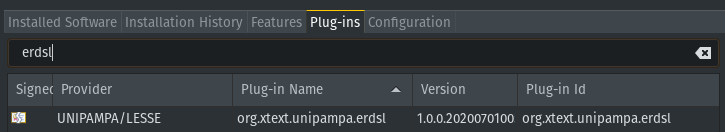
\includegraphics[width=0.48\textwidth]{images/PluginInstalado}
%     \caption{Installed solution plugin.}
%     \label{fig:pluginInstalado}
% \end{figure}

%After the plugin is integrated into RCP the
Figure \ref{fig:ERTextUso} shows a screenshot of the ERText. %, where it is possible to create data model files using our DSL.
This example is inspired on Chinook Sample Database (Repository: \url{github.com/lerocha/chinook-database}), and contains eleven (11) entities and ten (10) relationships, including generalization and specialization, a self-relationship and a ternary relationship.
ERText is embedded with design features assisted by real-time validation including: 
a) syntax highlighting  indicating syntax errors in writing time; 
b) code completion, and 
c) hovering, a feature that displays information about an item when the mouse cursor is placed over it.

In addition, although the definition of data types is not foreseen in the classic conceptual data model, for reasons related to the future intention to perform the generation of SQL commands, we decided to maintain this design decision in the grammar. 
%DD design decision.

\begin{figure}[!htb]
    \centering
    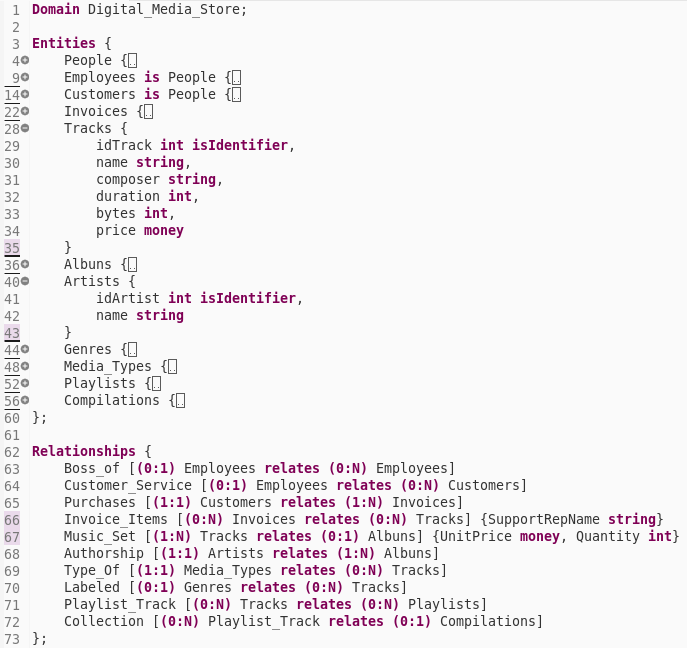
\includegraphics[width=0.48\textwidth]{images/ERTextUso4.png}
    \caption{Snippet of the solution being used.}
    \label{fig:ERTextUso}
\end{figure}

% A função para o mapeamento e geração do modelo lógico é executada automaticamente toda a vez que uma modelo é salvo.
% Na figura anterior pode-se observar os arquivos \textit{.html} na estrutura de diretórios na guia da esquerda, dentro da pasta \textit{src-gen}.
% Foram gerados arquivos com esse formato para uma melhor visualização a partir de marcações no texto.

%Previous figure highlighted the \texttt{.html} files available in the directory structure on the left tab, inside the \texttt{src-gen} folder.
Files with this format were generated for a better view from the text-markings using a model transformation of type model-to-text. 
These markings can be rendered by any browser, or even within the environment, increasing the power of understanding by the user.
The logical model mapping the conceptual data model, i.e., derived by the generator, is shown in Figure \ref{fig:modeloLogico}.

% Estas marcações podem ser renderizadas por qualquer navegador de Internet, ou mesmo dentro do próprio ambiente, aumentando o poder de compreensão por parte do usuário.
% O modelo lógico derivado pelo gerador que mapeia o modelo conceitual é apresentado na \autoref{fig:modeloLogico}.

\begin{figure}[!htb]
    \centering
    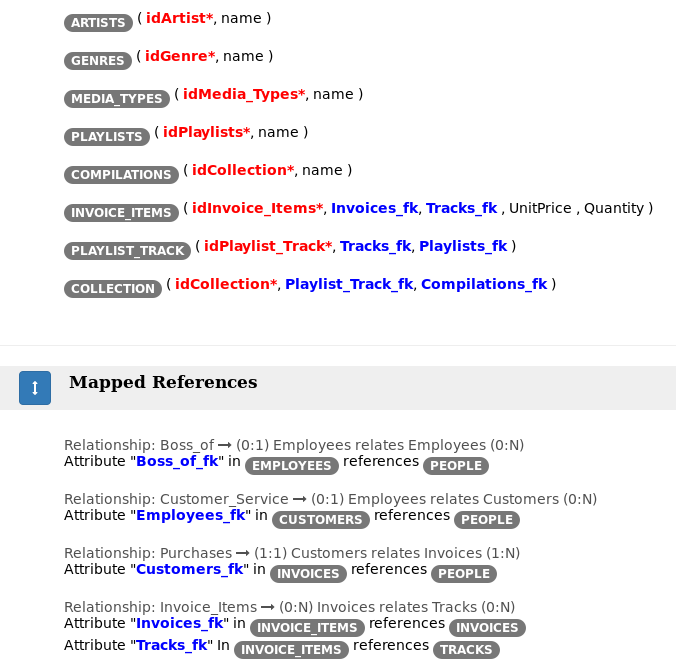
\includegraphics[width=0.48\textwidth]{images/ModeloLogico3.png}
    \caption{Snippet of the created logical model.}
    \label{fig:modeloLogico}
\end{figure}

The model-to-text transformation was mapped to the save event. Considering the exemplified model as input, this transformation results in a new model composed of fourteen (14) entities already having their inferred referential integrity, \textit{i.e.} the records that point to other records are already established.

In order to map and transform from a conceptual data model to a logical data representation of database, we adopted some assumptions proposed by Heuser \cite{Heuser:2009}.
The assumptions implemented so far can be summarized in:
\begin{inparaenum}[(i)]
\item column addition for 1:1 relationships;
\item column addition for 1:N relationships, and;
\item creation of own table for N:N relationships.
\end{inparaenum}

% Em relação ao conceito de generalização/especialização, também foi necessário assumir uma ideia inicial que teria que ser tomada como verdade.
% Segundo Heuser \cite{Heuser:2009}, para estes casos existe duas alternativas passíveis de serem derivadas. 
% A primeira recomenda o uso de uma única tabela para toda a hierarquia de entidades, ou seja, recomenda a fusão das tabelas.
% A segunda recomenda o uso de uma tabela por entidade modelada, desde que respeitado a integridade referencial, ou seja, as chaves primárias das entidades filhas devem apontar necessariamente para a chave primária da entidade pai. 
% No caso da ferramenta resultante neste trabalho, optou-se pela segunda alternativa.

%Regarding the generalization/specialization concepts, we also assume that an initial idea would have to be taken as truth.
According to Heuser \cite{Heuser:2009}, concerning generalization and specialization concepts, there are two alternatives that can be derived from a mapping for the transformation.
The first one recommends the use of a single table for the entire hierarchy of entities, \textit{i.e.} it advises merging the tables.
The second one suggests the use of a table by modeled entity, as long as respecting referential integrity, \textit{i.e.} the primary keys of the child entities must necessarily point to the primary key of the parent entity, creating a foreign keys references.
We chose the second alternative as assumption for this design decision.

% O gerador do modelo lógico foi desenvolvido com a GPL Xtend, e atualmente conta com cerca de quatrocentas linhas de código para realizar a transformação do modelo conceitual para o modelo lógico. 
The generator of the logical model was developed with GPL Xtend, and currently has about four hundred lines of code to carry out the transformation from the conceptual data model to the logical data model.

%#################################################
%#################################################
\section{\uppercase{Preliminary Evaluation}}
\label{sec:Evaluation}
%#################################################
%#################################################

% Esta seção descreve a avaliação preliminar conduzida para analisar a gramática proposta, visando assim o seu aperfeiçoamento em uma versão final na solução.
This section describes the preliminary evaluation conducted to analyze the proposed grammar, aiming to enhance it in a final version of the solution.

% Para tanto, foi estabelecido a utilização de um grupo focal, um método de pesquisa qualitativa que objetiva gerar feedback de um conjunto de pessoas em relação a um tema específico. 
For that, it was established the use of a focus group, a qualitative research method that aims to generate feedback from a group of people in relation to a specific topic.
% Essa abordagem é muito utilizada como uma atividade para pesquisa de mercado em diversas áreas, uma vez que pode cumprir papel importante apoiando pesquisas exploratórias.
This approach is widely used as an activity for market research in several areas, since it can play an important role in supporting exploratory research.
% O processo executado nessa etapa, expressado na Figura \ref{fig:focusGroup}, teve como base as diretrizes estabelecidas no trabalho de \cite{Kontio:2008}, as quais cobrem a aplicação desse método no contexto da Engenharia de Software.
Thus, starting from a previous investigation \cite{edmunds:2000,frisina:2006,tong:2007} the process carried out in this step, expressed in Figure \ref{fig:focusGroup}, was based on the guidelines established in the work of \cite{Kontio:2008}, which cover the application of this method in the context of Software Engineering.
%which contemplates the application of this method in the context of Software Engineering.

%The process performed in this step, expressed in Figure \ref{fig:focusGroup}, was based on the guidelines established in the work of Kontio \cite{Kontio:2008}, which cover the application of this method in the context of Software Engineering.

\begin{figure}[!htb]
    \centering
    

\tikzset{every picture/.style={line width=0.75pt}} %set default line width to 0.75pt        

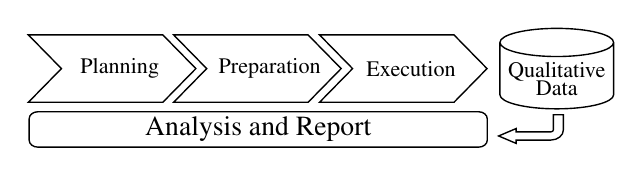
\begin{tikzpicture}[x=0.55pt,y=0.45pt,yscale=-1,xscale=1]
%uncomment if require: \path (0,300); %set diagram left start at 0, and has height of 300

%Chevron Arrow [id:dp3610810676849916] 
\draw  [line width=0.5]  (12.08,11.08) -- (100.42,11.08) -- (122.13,38.14) -- (100.42,65.19) -- (12.08,65.19) -- (33.8,38.14) -- cycle ;

%Flowchart: Magnetic Disk [id:dp3222965508094757] 
\draw  [line width=0.5]  (396.59,17.13) -- (396.59,59.14) .. controls (396.59,65.38) and (379.87,70.45) .. (359.24,70.45) .. controls (338.62,70.45) and (321.89,65.38) .. (321.89,59.14) -- (321.89,17.13)(396.59,17.13) .. controls (396.59,23.38) and (379.87,28.44) .. (359.24,28.44) .. controls (338.62,28.44) and (321.89,23.38) .. (321.89,17.13) .. controls (321.89,10.89) and (338.62,5.83) .. (359.24,5.83) .. controls (379.87,5.83) and (396.59,10.89) .. (396.59,17.13) -- cycle ;

%Chevron Arrow [id:dp9628056781818373] 
\draw  [line width=0.5]  (107.53,11.08) -- (195.86,11.08) -- (217.57,38.14) -- (195.86,65.19) -- (107.53,65.19) -- (129.24,38.14) -- cycle ;

%Chevron Arrow [id:dp8029700946101401] 
\draw  [line width=0.5]  (203.38,11.08) -- (291.71,11.08) -- (313.42,38.14) -- (291.71,65.19) -- (203.38,65.19) -- (225.09,38.14) -- cycle ;

%Rounded Rect [id:dp6923492778103744] 
\draw  [line width=0.5]  (12.59,78.48) .. controls (12.59,75.34) and (15.14,72.8) .. (18.27,72.8) -- (307.91,72.8) .. controls (311.05,72.8) and (313.59,75.34) .. (313.59,78.48) -- (313.59,95.52) .. controls (313.59,98.66) and (311.05,101.2) .. (307.91,101.2) -- (18.27,101.2) .. controls (15.14,101.2) and (12.59,98.66) .. (12.59,95.52) -- cycle ;

%Bend Arrow [id:dp33691381777556684] 
\draw  [line width=0.5]  (363.59,75.2) -- (363.59,87.28) .. controls (363.59,91.83) and (359.9,95.52) .. (355.35,95.52) -- (332.55,95.52) -- (332.55,98.21) -- (321.05,92.24) -- (332.55,86.26) -- (332.55,88.95) -- (355.35,88.95) .. controls (356.27,88.95) and (357.02,88.2) .. (357.02,87.28) -- (357.02,75.2) -- cycle ;

% Text Node
\draw (359.24,40.48) node  [font=\footnotesize] [align=left] {Qualitative};
% Text Node
\draw (359.24,53.97) node  [font=\footnotesize] [align=left] {Data};
% Text Node
\draw (163.09,87) node   [align=left] {Analysis and Report};
% Text Node
\draw (72.11,38.14) node  [font=\footnotesize] [align=left] {Planning};
% Text Node
\draw (170.63,38.14) node  [font=\footnotesize] [align=left] {Preparation};
% Text Node
\draw (263.45,38.14) node  [font=\footnotesize] [align=left] {Execution};


\end{tikzpicture}

    \caption{Focus Group Process~\cite{Kontio:2008}.}
    \label{fig:focusGroup}
\end{figure}

%#################################################
\subsection{Planning}
%#################################################

% Durante o planejamento foi definido um protocolo que deveria ser seguido.
During the planning stage, a protocol was defined that should be followed.
% Nesse protocolo, motivado pelo problema que era gerar uma versão definitiva da gramática da DSL proposta, foram criados os documentos necessários para sua execução: \textbf{(i)} Termo de Consentimento Livre e Esclarecido (TCLE); \textbf{(ii)} Glossário de Termos; \textbf{(iii)} Questionário de Perfil; \textbf{(iv)} Instrumentos da Discussão 1, 2 e 3; \textbf{(v)} Modelos das Gramáticas Avaliadas; \textbf{(vi)} Roteiro de Apresentação. 
In this protocol, motivated by the problem of generating a definitive version of the proposed DSL grammar, the necessary documents were created for its execution:
\textbf{(i)} Informed Consent Form (ICF); 
\textbf{(ii)} Glossary of Terms; 
\textbf{(iii)} Profile Questionnaire; 
\textbf{(iv)} Discussion Instruments 1, 2 and 3; 
\textbf{(v)} Models of the Grammars, and; 
\textbf{(vi)} Presentation Script.
% Todos os modelos dos documentos produzidos estão disponíveis em um repositório\footnote{https://github.com/anonymous/Focus-Group-Protocol} público.
All models of the documents produced are available in a public repository (Repository: \url{github.com/JonnathanRiquelmo/Focus-Group-Protocol} - in portuguese).

%#################################################
\subsection{Preparation}
%#################################################

% Tipicamente, as avaliações que utilizam grupos focais devem ser constituídas de quatro (4) a seis (6) grupos focais individuais para que o rigor científico seja considerado verdadeiramente alto. 
Typically evaluations using focus groups should consist of four (4) to six (6) individual groups to the scientific rigor to be considered high.
% O tamanho de cada grupo focal pode variar de três (3) a até doze (12) elementos, sendo mais comum esse número ficar entre quatro (4) e oito (8) participantes \cite{Kontio:2008}. 
The size of each group can vary from three (3) to twelve (12) elements, with the most common being a number between four (4) and eight (8) participants \cite{Kontio:2008}.

% Por questões de viabilidade de tempo e recursos humanos, para o presente estudo foi possível ser executado um (1) grupo focal. 
For the present study, it was possible to run one (1) focus group for reasons of time and human resources.
% Após a realização do convite houve a colaboração de treze (13) participantes, todos da área da Engenharia de Software. 
After the invitation, a total of thirteen (13) participants collaborated, all from the Software Engineering area.
% Desse total, três (3) participantes eram alunos de graduação, nove (9) eram mestrandos e um (1) doutorando. 
Of this total, three (3) participants were undergraduate students, nine (9) were master's students and one (1) doctoral student.

% Foi então aplicado o Questionário de Perfil, em que foi possível identificar que havia um nível equilibrado de conhecimento entre os participantes. 
The Profile Questionnaire was then applied, in which it was possible to identify that there was a balanced level of knowledge among the participants.
% Isso foi constatado pois todos já possuíam contato com DSL, tendo utilizado esse tipo de linguagem, ao menos, durante a graduação.
This was verified because everyone already had contact with DSL, having used this type of language, at least during graduation.
% Ainda foi informado que todo o processo seria gravado em áudio, fato com o qual todos concordaram.
It was also informed that the entire process would be recorded on audio, a fact that everyone agreed with it.

%#################################################
\subsection{Execution}
%#################################################

% O grupo focal foi realizado no segundo semestre de 2019, nas dependências de uma Instituição de Ensino Superior (IES), e teve duração duas (2) horas.
The focus group was held in the second half of 2019, on the premises of a higher education institution, and lasted for two (2) hours.
% Iniciando com a exposição do roteiro que deveria ser seguido, onde houve a apresentação do objetivo do grupo focal e os conceitos básicos envolvidos, aconteceu o pedido para que os participantes realizassem a leitura e assinatura do TCLE. 
Starting with the presentation script that should be followed, where there was the presentation of the focus group objective and the basic concepts involved, a request was made for the participants to read and sign the ICF.
% Com o documento preenchido, foi dado continuidade ao roteiro previsto.
With the signed ICF, we continued the planned script.

% A cada Instrumento de Discussão disponibilizado esperou-se até que os participantes respondessem de forma individual. 
For each discussion instrument available we waited until all the participants answered individually.
% Após, aconteceu uma discussão em grupo sobre o tema levantado.
Afterwards, there was a group discussion on the topic raised.
% Todo o processo foi gravado em áudio e teve o suporte dos três (3) pesquisadores envolvidos neste estudo.
The entire process was recorded in audio and had the support of the researchers involved in this study.
% Foi realizada também a transcrição das observações levantadas pelo debate que se seguiu, caracterizando assim as práticas de \textit{brainstorming}\footnote{\textit{Brainstorming} é uma técnica utilizada para propor soluções a um problema específico. Consiste em uma reunião, também chamada de tempestade de ideias, na qual os participantes devem ter liberdade de expor suas sugestões e debater sobre as contribuições dos colegas.} previstas em grupos focais.
A text transcription was made for the observations raised by the debate that followed, thus characterizing the brainstorming practices.

%#################################################
\subsection{Results Analysis}
%#################################################

% Segundo \cite{Kontio:2008}, a fase de análise e interpretação dos dados gerados constitui parte importante da pesquisa qualitativa, considerando o contexto, o comportamento e a percepção dos sujeitos. 
According \cite{Kontio:2008}, the analysis and interpretation stage of the generated data constitutes an important part of the qualitative research, considering the context, the behavior,  and the perception of the subjects.
% Para a fase de análise dos dados, o áudio foi analisado paralelamente as anotações realizadas.
For the data analysis stage the audio was analyzed in parallel to the taken notes.
% De posse desses materiais e das respostas dos participantes para cada instrumento de discussão, foi possível avaliar os resultados do grupo focal executado.
With these materials and the participant's responses to each discussion instrument, it was possible to evaluate the results of the executed focus group.

% Após a apresentação do roteiro preparado para o grupo focal, deu-se início as discussões dos três (3) instrumentos criados para a dinâmica.
After the presentation of the script prepared for the focus group, the discussions on the three (3) instruments created for the dynamics began.
% O primeiro instrumento continha a seguinte afirmação associada a uma escala Likert composta de níveis de concordância dispostos de um (1) a cinco (5), sendo um (1) indica discordância total e cinco (5) concordância total:
The first instrument contained the following statement, associated with a Likert scale, composed of levels of agreement, and arranged from one (1) to five (5), where one (1) indicates totally disagree and five (5) totally agree:
% \textit{\textbf{``Linguagens específicas de domínio com abordagem textual podem ser aplicadas na modelagem conceitual posto que conseguem descrever de forma rápida e concisa determinadas propriedades.
% Sendo assim, essas soluções podem ser utilizadas ou mesmo adaptadas de uma forma efetiva no que diz respeito a representação do domínio que modelam.''}}
\textit{\textbf{``Domain-specific languages with a textual approach can be applied in conceptual modeling as they can describe certain properties quickly and concisely.
Therefore, these solutions can be used or even adapted in an effective way with respect to the representation of the domain they model.''}}

% Após todos os participantes responderem o instrumento, foi aberto um momento de discussão entre todos. 
% Por não terem visto o modelo proposto de DSL, algumas dúvidas surgiram e os pesquisadores envolvidos procuraram sanar todas de forma a não influenciar as discussões seguintes.
After all participants answered the instrument, a moment of discussion was opened among all.
As they did not see the proposed DSL model, some doubts arose and the researchers involved sought to resolve all of them in order not to influence the following discussions.
% O debate prosseguiu com os participantes levantando possíveis vantagens de um modelo textual.
% Alguns citaram acreditar que essa abordagem poderia ser de mais fácil entendimento, porém que isso dependeria do usuário.
% Esta suposição incluiu dois prováveis tipos de perfis: analistas e desenvolvedores.
The debate continued with the participants raising possible advantages of a textual model.
Some said they believed that this approach could be easier to understand, but that it would depend on the user.
This assumption included two likely profile types: analysts and developers.
% O grupo chegou a conclusão que a abordagem poderia ser vista como mais produtiva por usuários de perfil desenvolvedor, mas menos proveitosa por aqueles que tivessem um viés mais analista em razão do seu nível de abstração em relação às abordagens gráficas.
% A Figura \ref{fig:disc1GPfocalGrafico} exibe a distribuição das respostas dos participantes para a primeira discussão.
The group came to the conclusion that the approach could be seen as more productive by users with a developer profile, but less profitable by those who had a more analytical bias due to their abstraction level in relation to graphic approaches.
Figure \ref{fig:disc1GPfocalGrafico} shows the responses distribution for the first discussion.

\begin{figure}[!htb]
    \centering
    % \includegraphics[width=0.8\textwidth]{img/QP1GrupoFocalGrafico.png}
    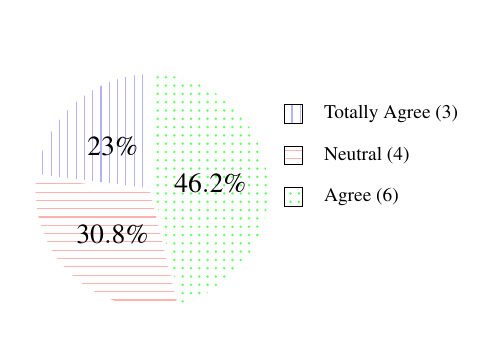
\begin{tikzpicture}
[
    pie chart,
    slice type={s1}{green!60}{dots},
    slice type={s2}{red!30}{horizontal lines},
    slice type={s3}{blue!30}{vertical lines},
    % slice type={s4}{purple}{bricks},
    % slice type={s5}{blue}{vertical lines},
    % slice type={s6}{cyan}{horizontal lines},
    % slice type={s7}{blue}{dots},
    pie values/.style={font={\normalsize}},
    scale=1.5,
]
    \pie{}{23/s3,30.8/s2,46.2/s1}
    \legend[shift={(1.2cm,1cm)}]{
        {Totally Agree (3)}/s3,
        {Neutral (4)}/s2, 
        {Agree (6)}/s1}
\end{tikzpicture}

% \begin{tikzpicture}
% \pie 
% [
%     radius = 2,
%     color={green!20, blue!20, orange!20}
% ]
%     {23/\textbf{Totally Agree (3)},
%     30.8/\textbf{Neutral (4)}, 
%     46.2/\textbf{Agree (6)}}
% \end{tikzpicture}
    \caption{Results of Discussion 1 - Focus Group.}
    \label{fig:disc1GPfocalGrafico}
\end{figure}

% Após, passou-se para a execução da discussão do segundo instrumento.
% O atividade era composta da seguinte pergunta:
Next, the discussion of the second instrument was carried out.
The activity consisted of the following question:
% \textit{\textbf{``Considerando que um modelo conceitual de banco de dados deve definir ao menos as entidades de domínio, seus atributos e o número de ocorrências (cardinalidade) possíveis de associações (relacionamento), como você definiria uma gramática básica (DSL) para a sua representação?''}}
\textit{\textbf{``Considering that a conceptual data model must define at least the domain entities, their attributes and the number of possible occurrences (cardinality) of associations (relationship), as you would define a basic grammar (DSL) for your representation?''}}

% Foi informado que os participantes poderiam conversar livremente durante toda a realização deste instrumento.
% Após cada um sugerir a sua sintaxe, houve debate e troca de informações sobre como estruturar melhor as informações. 
% A discussão foi focada principalmente em como representar as relações do modelo ER em uma sintaxe textual. 
It is important to mention that the participants could talk freely during the entire realization of this instrument.
After each one suggested its syntax, there was a debate and an information exchange on how to better structure the commands.
The discussion was mainly focused on how to represent the relations of the ER model in a textual syntax.

% A maior dificuldade se mostrou em como definir uma ordem. 
% Outro ponto que merece destaque foi quanto à cardinalidade, onde no geral seguiu-se a nomenclatura utilizada no diagrama original de Chen (\textit{e.g.} 0,1). 
% Entretanto, ao fim do instrumento houveram opiniões muito divergentes em relação à representação ideal. 
% Aparentemente, cada um teve uma visão distinta, alguns optando por incluir as relações dentro das entidades, e outros fora. 
The greatest difficulty observed is about how to define an order.
Another point worth mentioning was the cardinality, where in general the nomenclature used in Chen's original diagram (\textit{e.g.} 0,1) was followed.
However, at the end of the instrument, there were very divergent opinions in relation to the ideal representation.
Apparently, each had a different point of view, some choosing to include relationships within the entities, and others outside.
% Aconteceram também sugestões quanto às palavras-chave possíveis, como \texttt{Element}, \texttt{ElementFather}, \texttt{ElementSource}, \texttt{Type}, e \texttt{Referential}.
% Ainda, seis (6) participantes sugeriram o uso de ponto e vírgula (;) para separação das declarações de elementos, e todos os treze (13) preconizaram a utilização de símbolos como parênteses, colchetes e/ou chaves para agrupar conjuntos similares de elementos.	
There were also suggestions regarding possible keywords, such as \texttt{Element}, \texttt{ElementFather}, \texttt{ElementSource}, \texttt{Type}, and \texttt{Referential}.
Still, six (6) participants suggested the use of semicolons (;) to separate the declarations of elements, and all thirteen (13) recommended the use of symbols such as parentheses, brackets and/or keys to group similar sets of elements.

% Finalizada a dinâmica proposta, chegou-se ao último instrumento do grupo focal.
% Este artefato era composto de um exemplo de cada versão da gramática produzida preliminarmente para este trabalho \cite{Riquelmo:2019}.
% De posse das versões, foi pedido que os participantes realizassem a escolha entre as opções, apontando assim qual avaliavam como mais viável para modelagem ER.
% Também foi solicitado que fossem indicados os pontos positivos e negativos observados em cada modelo.
After the end of proposed dynamic, the last experimental instrument is executed: An artifact composed by an example of each grammar version produced preliminary for this work. 
%\cite{Riquelmo:2019}.
Based on both grammar versions, we asked the participants to choose between the options, thus indicating which one they evaluated as the most feasible for ER modeling.
In addition, we also requested to indicate the pros and cons observed in each model.
% O segundo modelo acabou por ser escolhido pela maioria, como pode ser observado na \ref{fig:disc3GPfocalGrafico}.
% Porém, ao final das discussões obteve-se um consenso de que a forma de definição de entidades do primeiro modelo e a disposição dos relacionamentos do segundo, em especial o uso das convenções nas cardinalidades, eram os mais adequados para a aplicação no ensino, indicando assim a necessidade de uma fusão de ambas as versões.
The second model was eventually chosen by the majority, as can be seen in Figure \ref{fig:disc3GPfocalGrafico}.
However, at the end of the conditions we reached a consensus: the way of defining entities of the first model and the disposition of relationships for the second, especially the use of conventions in cardinalities, are the most suitable for application in teaching-learning process, thus indicating the need for a merger of both versions.

\begin{figure}[!htb]
    \centering
    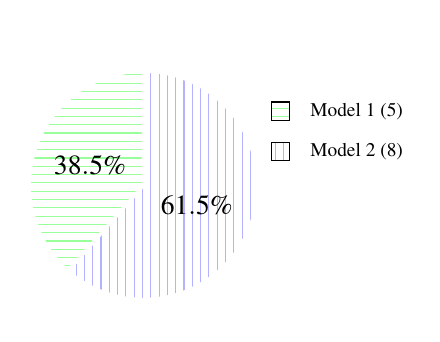
\begin{tikzpicture}
[
    pie chart,
    slice type={s1}{blue!30}{vertical lines},
    slice type={s2}{green!40}{horizontal lines},
    slice type={s3}{red!30}{dots},
    slice type={s4}{purple}{bricks},
    slice type={s5}{blue}{vertical lines},
    slice type={s6}{cyan}{horizontal lines},
    slice type={s7}{orange}{dots},
    pie values/.style={font={\normalsize}},
    scale=1.45,
]
    \pie{}{38.5/s2,61.5/s1}
    \legend[shift={(1.2cm,1cm)}]{
        {Model 1 (5)}/s2,
        {Model 2 (8)}/s1}
\end{tikzpicture}

% \begin{tikzpicture}
% \centering
% \pie
% [
%     radius = 2,
%     color={green!20, orange!20}
% ]
%     {38.5/\textbf{Model 1 (5)},
%      61.5/\textbf{Model 2 (8)}}
% \end{tikzpicture}
    \caption{Results of Discussion 3 - Focus Group.}
    \label{fig:disc3GPfocalGrafico}
\end{figure}


%#################################################
%#################################################
\section{\uppercase{Threats to Validity}}
\label{sec:threats}
%#################################################
%#################################################

% Aiming that the evaluation has a valid result for the proposed focus group, it was necessary to analyze and discuss some threats to validity, as well as the strategies used to mitigate them.
For the list of possible threats, the topics and recommendations raised in the work of \cite{Wohlin:2012} were used.
These threats followed a pattern and were divided into four (4) categories as follows.
%, namely: construct validity, internal validity, external validity and conclusion validity.

% \subsection{Validade do Construto}
% A validade do construto diz respeito ao design do experimento e a fatores sociais.
% \begin{inparaenum}
% (i) \textit{\textbf{Explicação pré-operacional inadequada}}: Esta ameaça está relacionada com o fato do grupo focal não ter o objetivo dos artefatos suficientemente definidos antes de serem traduzidos em medidas ou tratamentos. 
% (ii) \textit{\textbf{Interação de diferentes tratamentos}}: Se os sujeitos estiverem envolvidos em mais de um estudo, os tratamentos dos diferentes estudos poderão interagir e reverberar nos resultados finais. Todos os sujeitos fizeram apenas esse grupo focal na época de sua realização. 
% \end{inparaenum}
%\subsection{Construct Validity}
\textbf{Construct Validity}: concerns the experimental design and social factors.
(i) \textit{Inadequate Preoperational Explication}: This threat is when the focus group may not have the objective of the artifacts sufficiently defined before they are translated into measures or treatments.
(ii) \textit{Interaction of different treatments}: If the subjects are involved in more than one study, the treatments of the different studies may interact and reverberate in the final results. 
All subjects did just this focus group at the time of realization.

% \subsection{Validade Interna}
% \begin{inparaenum}
% (i) \textit{\textbf{História}}: Há o risco de algum período temporal específico ter influência na realização do experimento. Para mitigar esta ameaça, e em razão do grupo focal ser realizado em ambiente acadêmico, todo o processo foi executado mediante aviso dos participantes quanto a um período em que todos não estivessem necessariamente sobrecarregados com atividades acadêmicas \textit{e.g.} provas e trabalhos.
% (ii) \textit{\textbf{Testes}}: Se os testes forem repetidos, os sujeitos podem responder de maneira diferente em momentos diferentes, pois sabem como o teste é realizado. Se houver necessidade de familiarização com os testes, é importante que os resultados do teste não sejam devolvidos ao sujeito, para assim não apoiar o aprendizado não intencional. Não houve necessidade de repetição das atividades, uma vez que as mesmas foram executadas uma vez por cada participante.
% (iii) \textit{\textbf{Instrumentação}}: Essa ameaça está relacionada aos artefatos usados para a execução da experiência, como formulários de coleta de dados, etc. Se estes foram mal projetados, a experiência é afetada negativamente. Para combater essa ameaça, todos os artefatos foram verificados e validados previamente em reuniões entre os pesquisadores envolvidos neste trabalho.
% \end{inparaenum}

% \subsection{Internal Validity}
\textbf{Internal Validity}: are influences that can affect independent variables in relation to causality, without the researcher's knowledge.
(i) \textit{History}: There is a risk that a specific time period will influence the experiment. In order to mitigate this threat
% , and because the focus group is carried out in an academic environment, 
the entire process was carried out upon the participants' notice of a period when everyone was not necessarily overwhelmed with academic activities \textit{e.g.} tests and assignments.
(ii) \textit{Tests}: If the tests are repeated, the subjects may respond differently at different times, as they know-how the test is performed. 
% If there is a need to familiarize with the tests, it is important that the test results are not returned to the subject, so as not to support unintentional learning. 
There was no need to repeat the activities, since they were performed once by each participant.
(iii) \textit{Instrumentation}: This threat is related to artifacts used for the execution of the focus group, such as data collection forms, etc. If these are poorly designed, the experience is negatively affected. To combat this threat all artifacts were previously checked and validated at meetings among the researchers involved in this work.

% \subsection{Validade Externa}
% \begin{inparaenum}
% (i) \textit{\textbf{Sujeitos}}: Os sujeitos selecionados para o grupo focal podem não representar um grupo significativo para a área de estudo. Buscando tentar mitigar essa ameaça foi realizado com participantes da área de Engenharia de Software e Ciência da Computação, e logo, inseridos no contexto de uso da modelagem conceitual de BD relacionais. Porém, o fato da amostra ser de apenas um grupo focal é uma ameaça indicada na literatura. Não foi possível mitigar este fato.
% (ii) \textit{\textbf{Interação dos sujeitos com os artefatos de avaliação}}: Essa é a ameaça relacionada a aplicação dos artefatos de avaliação do grupo focal com os sujeitos. Dependendo do momento isto pode afetar os resultados. Se, por exemplo, um questionário for realizado alguns dias após a execução do grupo focal, as pessoas tendem a responder de maneira diferente do que fariam momentos após as atividades. Todos os instrumentos foram realizados na mesma sessão.
% \end{inparaenum} 

%\subsection{External Validity}
\textbf{External Validity}: are conditions related to replication of the evaluation.
(i) \textit{Subjects}: The subjects selected for the focus group may not represent a significant group for the study area. In an attempt to mitigate this threat it was carried out with participants from the area of Software Engineering and Computer Science, inserted in the context of the use of conceptual modeling of databases. 
However, the fact that the sample is of only one focus group is a threat indicated in the literature. It was not possible to mitigate this fact.
(ii) \textit{Interaction of subjects with assessment artifacts}: This is the threat related to the application of the assessment artifacts 
%of the focus group 
with the subjects. Depending on the moment this can affect the results. If, \textit{e.g.} a questionnaire is carried out a few days after the execution of the focus group, people tend to answer differently than they would do moments after the activities. All instruments were performed in the same session.

% \subsection{Validade da Conclusão}
% \begin{inparaenum}
% (i) \textit{\textbf{Confiabilidade dos resultados}}: A confiabilidade dos resultados obtidos tem impacto direto na validade do grupo focal como um todo. Por ser uma avaliação com maior foco qualitativo, esta ameaça não pôde ser mitigada em razão da subjetividade inerente às resposta dos sujeitos em tais avaliações.
% \end{inparaenum}

%\subsection{Conclusion Validity}
\textbf{Conclusion Validity}: are related to issues affecting the ability to infer a correct conclusion about the relationship between treatments and results of an evaluation.
(i) \textit{Reliability of Results}: This threats obtained has a direct impact on the validity of the focus group as a whole. As it is an assessment with a greater qualitative focus, this threat could not be mitigated due to the subjectivity inherent in the subjects' responses in such assessments.
(ii) \textit{Evaluation Environment}: The assessment should be carried out in a controlled environment, trying to avoid external influences. 
To mitigate this possible threat, participants were instructed that conversations outside the scope of the focus group could not take place during the entire duration of the activities, as well as leaving the environment or accessing electronic devices. 
% However, for the comfort of the subjects, everyone was advised that they could interrupt their participation at any time they wanted.

%#################################################
%#################################################
\section{\uppercase{Conclusions}}
\label{sec:conclusion}
%#################################################
%#################################################

In this study, the requirements, the design decisions, the architecture, and the ERText tool were exposed.
XText proved to be an LW capable of meeting the needs of the project.
% , providing full support for the creation of grammars with BNF notation, a meta-syntax widely used to express context-free grammars as in the structures of programming languages in general.
Using this framework, a DSL was defined and implemented as an integrated plugin in an Eclipse RCP, thus generating the ERText tool.

In this way, the modeling process with the newly created language gained native features such as code completion, formatting, validation based on the restrictions described in the grammar, and syntax highlighting.
It is important to note that the plugin could only be tested due to the native integration provided by XText with EMF, a set of Eclipse features to represent models and generate code. %equivalent code.
%Colocar aqui um parágrafo que resume os estudos de avaliação realizados na ERText, desde a concepção até o teste final.

With the investigation of the scientific literature and the experience acquired mainly during the design stage of the textual DSL development, we can also mention the occurrence of a preliminary evaluation of a prototype with 13 participants.
With the feedback obtained, it was possible to carry out the evolution of development and the definition of an experimental protocol to perform an empirical evaluation of the product developed.

Consequently, a controlled experiment (\url{doi.org/10.5281/zenodo.4064991}) was carried out with 27 participants, all students of different levels and belonging to SE area.
This evaluation used two treatments, one with a graphical approach and the other with ERtext, with the groups of subjects randomly balanced.
With the data collected it was possible to execute a quantitative and qualitative analysis of the tool's viability.
The results obtained show evidence that, when performing modeling tasks with both approaches, there is less effort associated with the graphical approach.
We believe this is due to the fact that the textual approach to conceptual modeling was not familiar to the subjects of the experiment.
On the other hand, the performance was very similar regarding the quality of the models made in both tools, indicating some potential for competition of the proposal concerning to the graphical approach tools.

As future work, the solution is expected to generate SQL code for different technologies (\textit{e.g.} MySQL, PostgreSQL), including as an improvement not only the generation of DDLs but also, for example, stored procedures of CRUD operations for each modeled entity. 
Besides, we intend to generate Object Relationship Mapping (ORM) input structures, for instance Hibernate and Entity Framework.

Finally, the project for this solution is publicly available under the EPL-2.0 license in the GitHub repository (Repository: \url{github.com/ProjetoDSL/ERDSL}), 
belonging to 
%our Research Lab from a public university.
the Laboratory of Empirical Studies in Software Engineering (LESSE) research group of Unipampa.

% \vfill
% \section*{\uppercase{Acknowledgements}}
% \noindent This research is partially funded by FAPERGS N\textsuperscript{\underline{o}}04/2019.

\bibliographystyle{apalike}
{\small
\bibliography{0Bib}}


% \section*{\uppercase{Appendix}}

% \noindent If any, the appendix should appear directly after the references without numbering, and not on a new page. To do so please use the following command:
% \textit{$\backslash$section*\{APPENDIX\}}

\end{document}

